\chapter{Scripts, input files and directories\label{chap:general}}
%-----------------------------------------------------------

This chapter starts with the description of the scripts used by \diva, then input files required for simple 2-D analysis are presented here. 
Basically, only three files are needed as input:

\begin{enumerate}
\item a file containing the data (\file{data.dat})
\item the specification of the domain of analysis (\file{coast.cont}) and 
\item the list of the parameters used during the analysis (\file{param.par}).
\end{enumerate}


\minitoc

\newpage % 


\paragraph*{Convention:} \diva works with decimal numbers\\ 
represented with\quad \textbf{.}\quad  not \quad \textbf{,}

\btips
Use unix command \command{sed} to replace \textbf{,} by \textbf{.}:
\begin{lstlisting}[style=Bash]
[charles@gher13 Software] cat file1.dat | sed s/,/./g > file2.dat
\end{lstlisting}

where: \file{file1.dat} is the old file and \\
\hphantom{where:} \file{file2.dat} is the file where the replacement has been made.
\etips


\btips
Use editor \textsl{vi} to replace \textbf{,} by \textbf{.}:

Simply type:
\begin{lstlisting}[style=Bash]
[charles@gher13 Software]$ vi file1.dat
:,$s/,/./g
\end{lstlisting}

\etips



\section{List of 2-D tools}
%-------------------------

\subsection{Operations on data}

\begin{description}
\item[\command{divabin}:] bins the data in order to improve the quality of the optimized parameters (CL and SNR).
\item[\command{divaanom}:] computes the difference between the data and the provided reference field. 
\item[\command{divadataclean}:] eliminates all data that fall outside the bounding box of the contours.
\item[\command{divadatacoverage}:] Writes Relative Length (RL) (\file{RL.dat} and \file{RLInfo.dat}) field based on data coverage and data density field (\file{DATABINS.dat}).
\item[\command{dvncmask2RL}:] Writes Relative Length (RL) (\file{RL.dat} and \file{RLInfo.dat}) field based on a given mask on the domain.  
\end{description}


\subsection{Parameter estimation}

\begin{description}
\item[\command{divabestguess}:] provides estimates for the correlation length and the signal-to-noise ratio with methods chosen according to the number of data.
\item[\command{divacv}:] performs ordinary cross-validation.
\item[\command{divacvclasses}:] performs ordinary cross-validation by setting aside all data from a given class (e.g., specific year) and comparing the analysis to them.
\item[\command{divacvrand}:] performs cross-validation by taking out several points at once to calculate error estimates and repeat the exercise several times to make estimates robust.
\item[\command{divafit}:] estimates the correlation length by fitting the data correlation function to the theoretical kernel. \index{Correlation length}
\item[\command{divagcv}:] estimates the signal-to-noise ratio by performing a generalised cross-validation.\index{Signal-to-noise ratio}
\item[\command{divagcvalex}:] 
\item[\command{divaguesssn}:] 
\item[\command{divasnbygrid}:] creates a grid with noise level and data weights.
\end{description}

\subsection{Contours and mesh}

\begin{description}
\item[\command{divacc}:] check the consistency of the initial contour file.
\item[\command{divacoa2cont}:] converting ODV-format coastlines to \diva-format coastlines.
\item[\command{divacont}:] creates the contours from a given bathymetry and a selected depth levels.
\item[\command{divacont2grid}:] translate contours into gridded format.
\item[\command{divamesh}:] generates the finite-element mesh.
\end{description}

\subsection{Analysis}

\begin{description}
\item[\command{divabigtest}:] performs a test with a very large number of data points.
\item[\command{divacalc}:] performs the \diva analysis.
\item[\command{divadetrend}:] performs an analysis with the detrending option activated.
\item[\command{divadress}:] performs a complete analysis: cleaning (divaclean), mesh generation (divamesh), analysis (divacalc), outliers detection (divaqcbis) and outliers removal (dvoutlierclean)
\item[\command{divaintegral}:] compute the integral of the treated variable of the considered domain.
\item[\command{divamultivar}:] performs an analysis with the multivariate approach.
\item[\command{divarefe}:] computes a reference field with a semi-normed analysis with an increased value for $L$.
\item[\command{divaseminorm}:] performs an analysis with a semi-normed reference field: computes the reference field (\command{divarefe}), computes the anomalies with respect to the reference field (\command{divaanom}), makes the analysis (\command{divacalc}) and add the reference field to the obtained analysis (\command{divasumup}).
\item[\command{divasumup}:] performs the last step of a semi-normed analysis: the sum of background field and analysed anomaly field.
\end{description}

\subsubsection{Analysis: using relative length field}

\begin{description}
\item[\command{divadatacoverage}:] Writes in \directory{input} Relative Length (RL) field based on data coverage. RL fields are used to perform an analysis when they are present in  \directory{input}.
\item[\command{dvncmask2RL}:] Writes Relative Length (RL) field based on a given netcdf mask file of the domain. It uses the file \file{mask.nc} if present in \directory{input} and writes \file{RL.dat} and \file{RLInfo.dat} to \directory{input} directory.

\end{description}


\subsection{Quality control and error field}

\begin{description}
\item[\command{divacpme}:] computes de the clever poor man's error.
\item[\command{divaexerr}:] advanced method to compute the exact error field.
\item[\command{divaqc}, \command{divaqcbis}, \command{divaqcter}:] performs quality control on data (see Section~\ref{secdivaqc}).
\end{description}

\subsection{Misc}

\begin{description}
\item[\command{divaclean}:] cleans up the working directories by removing \file{fort.*} files from \directory{divawork} and \directory{meshgenwork}, as well as output files from \directory{output}.
\item[\command{divagnu}:] prepares the plot of outputs using Gnuplot.
\item[\command{divaload}:] load the input files from a given directory.
\item[\command{divasave}:] saves the output files in a given directory.
\end{description}

%--------------------
\section{Input files\label{sec:diva2Dinput}}
%--------------------

\subsection{Contour\label{contourdiva}}
%--------------------------------------

\index{Contours}
The contour file (\file{coast.cont}) delimits the region where the analysis has to be performed, i.e., it specifies the boundary between land and sea. The file is defined this way:
\begin{enumerate}
\item The first line indicates the number of contours ($M$) in the region of interest.
\item The second line tells the number of points ($N_{1}$) in the first contour.
\item The next $N_1$ lines are the coordinates of the points of the first contour. The convention for the contour is that \textit{the land is on the right when you follow the points successively}. The contour is automatically closed, meaning that the last point of a given contour is be from the first one. 
\item The following line is the number of points ($N_{2}$) of the second contour.
\item \ldots
\item The last $N_M$ lines are the coordinates of the points of the last contour.
\end{enumerate}

\begin{exfile}[htpb]
\begin{footnotesize}
\texttt{2\\
4\\
0 0\\
100 0\\
100 80\\
0 80\\
4\\
60 40\\
80 40\\
80 60\\
60 60} 
\end{footnotesize}
\caption{coast.cont\label{ex:coast.dat}}
\end{exfile}

Here, the contour is made up of 2 sub-contours: 
\begin{itemize}
\item the first one with 4 points (and 4~edges): $(0,0)$, $(100,0)$, $(100,80)$ and $(0,80)$. It is the main contour.
\item the second one with also 4 points. It is the interior contour (island).
\end{itemize}
In realistic application, the contours are more complex: they have more sub-contours (islands, interior seas), and each sub-contour is made up of more points. 

\begin{figure}[H]
\centering 
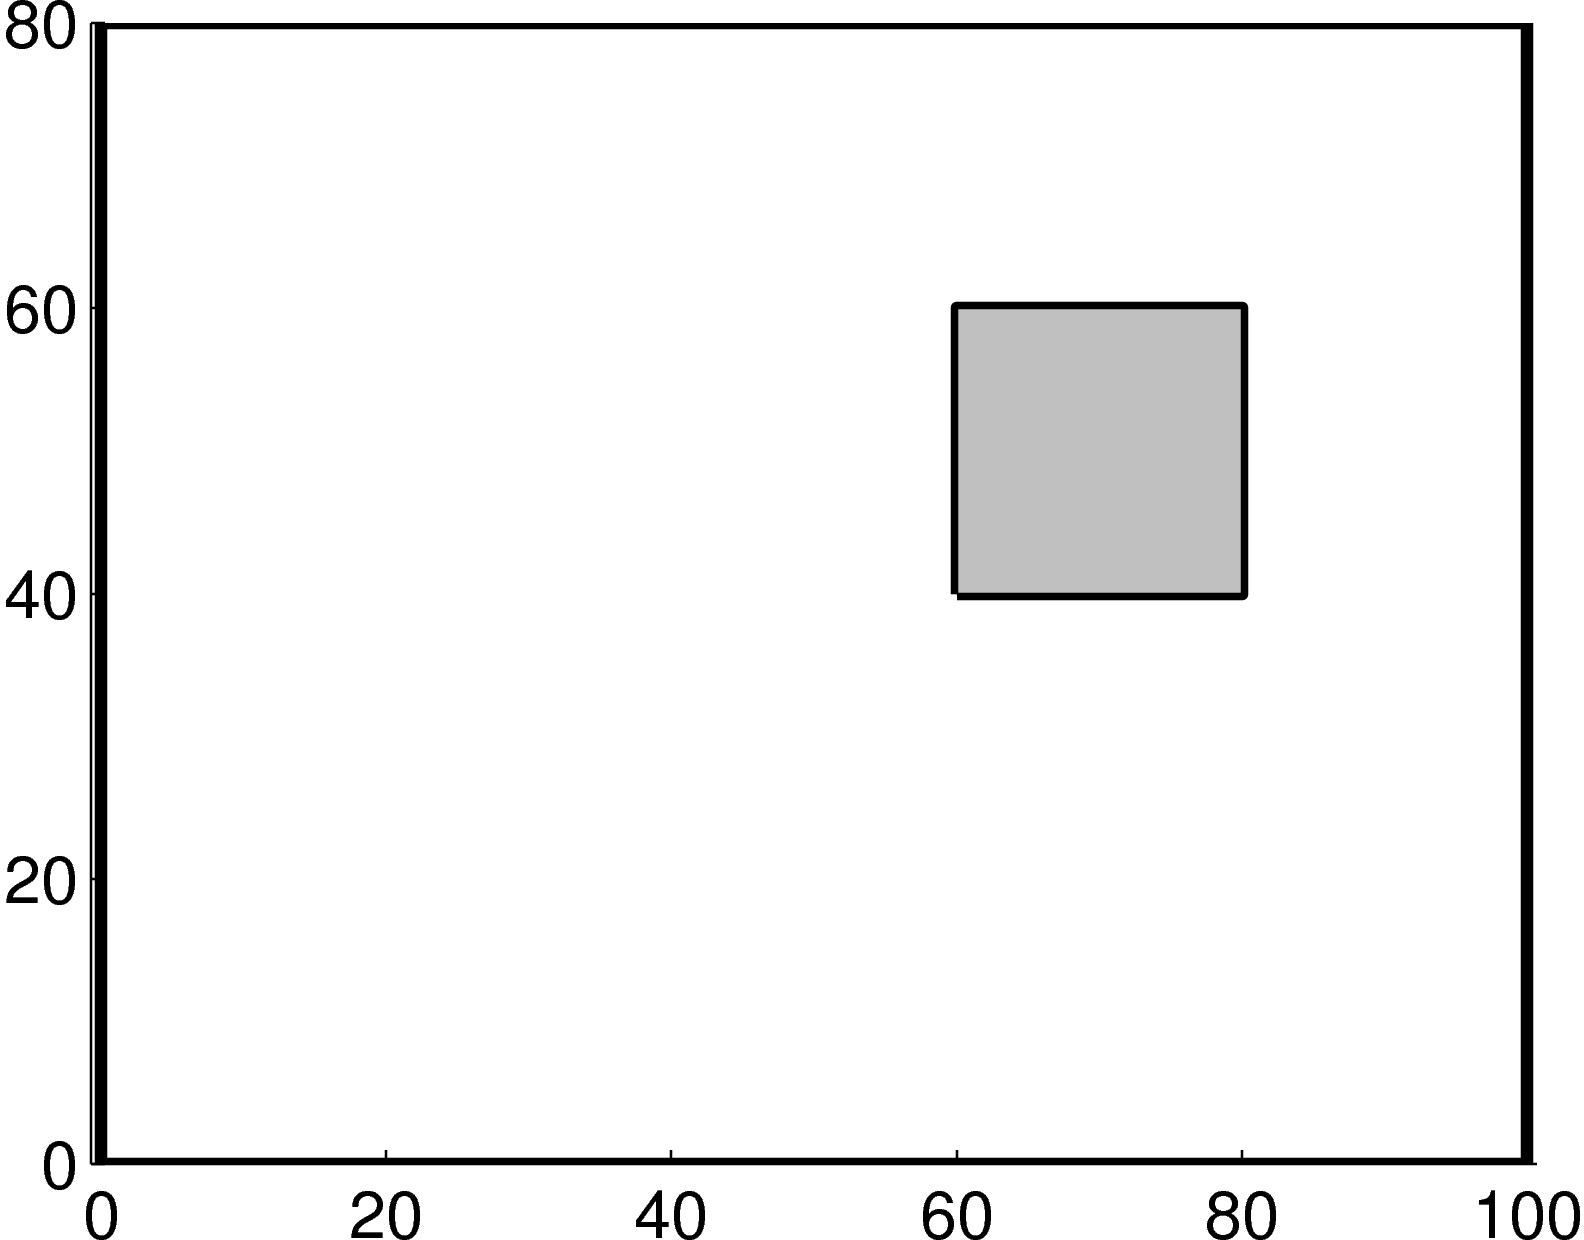
\includegraphics[width=.5\textwidth,bb=110 268 492 576]{coast_cont_fig}
\caption{Example of a contour file and its graphical representation.}
\end{figure}

%---------------
\subsection{Data\label{sec:dataformat}}
%----------------

\index{Data}
The data file (\file{data.dat}) contains at least three columns: 
\begin{enumerate}
\item the $x-$coordinate (usually the longitude, but can also be an horizontal distance in $km$, or any coordinate).
\item the $y-$coordinate (usually the latitude).
\item the data value.
\end{enumerate}
\begin{itemize}
\item The fourth column [optional] indicates the weight\index{Weight} of the each data point. If this column is empty, the fourth column is assumed to take the value $1$. 
\item If there are more than four columns, columns 5 and higher are not used by the software, except if you want to use the detrending tool (Section~\ref{sec:detrending})\index{Detrending}. 
\end{itemize}

\begin{exfile}[htpb]
\begin{footnotesize}
\texttt{20 10 3\\
60 20 -2\\
30 50 0\\
40 70 -1\\
70 70 -2\\
85 55 4\\
90 10 2\\
70 35 -4} 
\end{footnotesize}
\caption{data.dat\label{ex:data.dat}}
\end{exfile}


\begin{figure}[H]
\centering
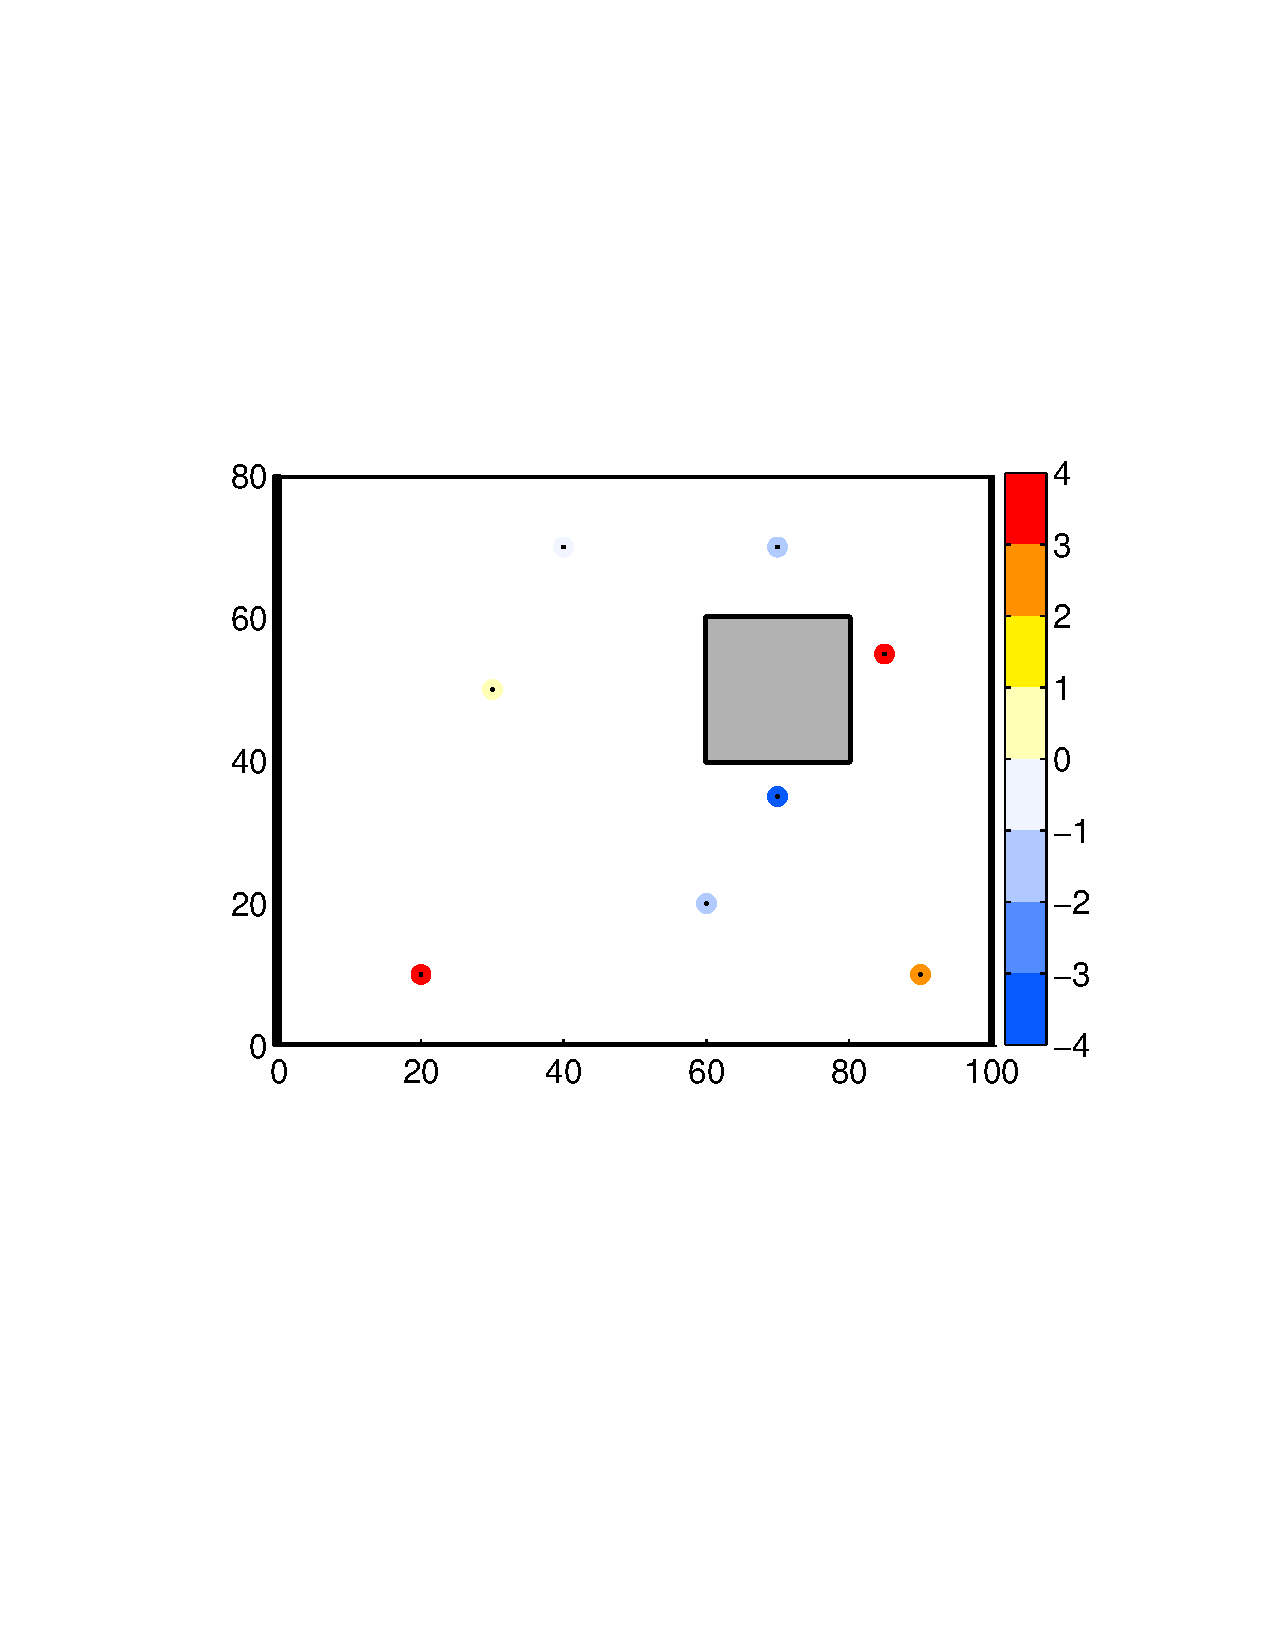
\includegraphics[width=.55\textwidth,bb=110 268 525 577]{data_dat_fig}
\caption{Example of a data file and its graphical representation.}
\end{figure}




\subsection{Parameters\label{sec:param.par}}
%-------------------------------------------

\index{Parameters}
The file \file{./input/param.par} specifies the main analysis parameters and options of \diva. A clear understanding of is essential for a proper use of the software. A description of each parameter is provided below the example file.

\begin{exfile}[htpb]
%\begin{footnotesize}
\begin{verbatim}
# Correlation Length lc
0.2
# icoordchange
0
# ispec
11
# ireg
0
# xori
0
# yori
0
# dx
0.02
# dy
0.02
# nx
51
#ny
51
# valex
-99
# snr
1.0
# varbak
1.0
\end{verbatim}
%\end{footnotesize}
\caption{param.par\label{paramfile}}
\end{exfile}


\subsubsection{\texttt{Lc}}
% ------------------------

The global correlation length $L$ \index{Correlation length} used for the analysis (see Section~\ref{sec:parammeaning} for 
the physical meaning). It has to be defined as a real positive number. Note that the length of the finite-elements 
will be computed according to the value of $L$.

As a first guess, you can use a value between a tenth of the domain size and the domain size, in order to avoid
getting into memory troubles due to a too fine mesh. Later, you can change this value if it seems interesting (via optimization).

\subsubsection{\texttt{icoordchange}\label{sec:icoord}}
%---------------------------------------------------


Specifies the desired type of coordinate system:\\

\texttt{icoordchange} \begin{minipage}[t]{.7\textwidth} = $0$ if no change is necessary (same coordinates as data);\\
                                                        = $1$ if data positions are given in degrees and if you want to use real distances;\\
                                                        = $2$ if data positions are given in degrees, you want to use real distances, and your domain extends on a wide span of latitude                                                           (uses a cosine projection);\\
                                                        = $-xscale$ to scale $x$ coordinates by a factor $xscale$ before doing anything (for vertical sections: see Section~\ref{sec:cruise})
                      \end{minipage}
                      
                      
\subsubsection{\texttt{ispec}}
%--------------------------

Four base-values specify the required error outputs:\\

\texttt{ispec}       = 0\qquad: no error field requested\\
\hphantom{\texttt{ispec}}  = 1\qquad: gridded error field specified by \texttt{xori}, \texttt{yori}, \texttt{nx} and \texttt{ny}; \\
\hphantom{\texttt{ispec}}  = 2\qquad: errors at data locations;\\
\hphantom{\texttt{ispec}}  = 4\qquad: errors at locations listed in \file{valatxy.coord}.

Then you can combine these four values to obtain several error outputs: \index{Error}

\examples\\
\texttt{ispec}             = 3 (=1+2)\hphantom{+4} \qquad \begin{minipage}[t]{.7\textwidth}means you want gridded error field as well as errors at data locations;\end{minipage}\\ 
\texttt{ispec}             = 7 (=1+2+4) \qquad means you want the three error files.


From there several variants can be specified:

For computing errors with the real covariance function (Section~\ref{sec:realcovariance}), simply multiply the \texttt{ispec} value by $-1$:

\example\\
\texttt{ispec}             = -7 \qquad \begin{minipage}[t]{.7\textwidth}{means you want the three error files computed with the help of the real covariance function.}\end{minipage}


For computing errors with the real covariance function using boundary effects (Section~\ref{sec:realcovariance}), simply add $-10$ to a negative \texttt{ispec}:

\example\\
\texttt{ispec}             = -17 \qquad \begin{minipage}[t]{.7\textwidth}{means you want the three error files computed with the help of the real covariance function and boundary effects.}\end{minipage}


A \textit{poor man's} error estimate (quick and underestimated error field, Section~\ref{sec:poormans}) is available by adding $+10$ to the positive base \texttt{ispec} value:

\example\\
\texttt{ispec}             = 16 \qquad \begin{minipage}[t]{.7\textwidth}{means you want errors at data locations and at points listed in \file{valatxy.coord} computed with the \textit{poor man's} error estimate.}\end{minipage}



Adding $+100$ to the base \texttt{ispec} activates  the clever poor man's error calculation and launches automatically \command{divacpme}

\example\\
\texttt{ispec}             = 116 \qquad \begin{minipage}[t]{.7\textwidth}{means you want errors at data locations and at points listed in \file{valatxy.coord} computed with the \textit{clever poor man's} error estimate.}\end{minipage}

Adding $-100$ to a negative \texttt{ispec} activates the almost exact error calculation and launches automatically \command{divaexerr}

\example\\
\texttt{ispec}             = -106 \qquad \begin{minipage}[t]{.7\textwidth}{means you want errors at data locations and at points listed in \file{valatxy.coord} computed with the almost exact error estimate.}\end{minipage}



\example\\
\texttt{ispec}             = -117 \qquad \begin{minipage}[t]{.7\textwidth}{means you want errors everywhere computed with the almost exact error estimate using the background covariance with boundary effects.}\end{minipage}






\subsubsection{\texttt{ireg}}

Specification of the background field which is subtracted from the data field (Section~\ref{sec:backgroundfield}).

\texttt{ireg}             = 0 \qquad: no background field is subtracted (assuming data are already anomalies); \\
\hphantom{\texttt{ireg}}  = 1 \qquad: the data mean value is subtracted;\\
\hphantom{\texttt{ireg}}  = 2 \qquad: the linear regression of the data (plane) is subtracted.

\subsubsection{\texttt{xori/yori, nx/ny}}

\texttt{xori/yori} indicate the coordinates of the first grid point while \texttt{nx/ny} indicate the number of grid points in \texttt{x/y} directions.



\subsubsection{\texttt{valex}}
%-----------------------------

Exclusion value: value used to fill the output matrix when a point corresponds with land. Any value is accepted, but the user has to ensure that the exclusion value cannot be a value obtained by the interpolation of the measurements. 


\subsubsection{\texttt{snr}}
%---------------------------

Signal-to-noise ratio of the whole dataset (Section~\ref{sec:formulation}). It has to be defined as a real positive number (as the correlation length).\index{Signal-to-noise ratio}

\subsubsection{\texttt{varbak}}
%------------------------------

Variance of the background field. 

\subsection[Additional points of analysis]{Locations of additional points where analysis is required (optional)}
%--------------------------------------------------------------------------------

The file \file{valatxy.coord} is a two-column list of locations where you want the analysis to be performed (in addition to the regular grid defined in \file{param.par}).  

\begin{exfile}[htpb]
\begin{footnotesize}
\texttt{20 20 0\\
60 10\\
40 40} 
\end{footnotesize}
\caption{valatxy.coord\label{ex:valatxy}}
\end{exfile}

If they exist, columns 3 and higher are not used.


\section{Working directories (2-D analysis)}
% ------------------------------

For 2-D analysis, the main working directory is \directory{divastripped}. Inside it, we have:
\begin{lstlisting}[style=Bash]
[charles@gher13 divastripped] tree -d -L 2
.
|-- divawork
|   `-- sub
|-- gnuwork
|   |-- gnuplottools
|   `-- plots
|-- input
|-- meshgenwork
`-- output
    |-- ghertonetcdf
    `-- meshvisu

10 directories
\end{lstlisting}


\begin{description}

\item[\directory{divawork}] is where the intermediate files are produced.
\item[\directory{gnuwork}] contains the scripts for generating the plots with Gnuplot. These plots will be located in the sub-folder \directory{plots}.
\item[\directory{input}] contains the input files presented in this section.
\item[\directory{divawork}] is the working directory for the mesh generation.
\item[\directory{output}] contains the analysis results. In \directory{ghertonetcdf}, one can find the output in NetCDF format (file \file{results.nc}), while \directory{meshvisu} stores the files that describe the mesh.
\end{description}
